\documentclass[a4paper,12pt]{article}
    \usepackage{amsmath}
    \usepackage{graphicx}
    \usepackage{multirow}
    \usepackage[top=1.1in, bottom=1.1in, left=1.15in, right=1.15in]{geometry}
    \usepackage{fancyhdr}
    \usepackage{relsize}
	\makeatletter
    \setlength{\@fptop}{0pt}
    \makeatother
\title{\Huge{\textbf{Research seminar and journal club - Assignment Report}}\\[0.5em]\smaller \textbf{TU Bergakademie Freiberg\\SS-18/19}}
\author{Arun Prakash Ganapathy\\
\small{Mat.Nr. 63876}\\
\small{E-Mail: arun-prakash.ganapathy@student.tu-freiberg.de}
}
\date{}


\begin{document}
\maketitle
\newpage

\section{Introduction:}
\indent\indent In macroscopic scale the plastic deformation appears smooth in stress-strain curve but in microscopic scale the deformation happens intermittently i.e.,it takes place through bursts. This caused due to dislocation avalanches. Crystal deform by dislocation multiplication and avalanches. Avalanches starts with dislocation accumalation and formation of dislocation bands. The dislocation gets piled up before these bands whose giveaway triggers avalanches(like opening a flood gate). The dislocation avalanches can be well explained by a phenomenon called Self-Organised Criticality(SOC). It states that  any slowly driven non-equilibrium systems self-organise themselves in a critical state where anything can happen within well defined statistical laws. They are scale-free, intermittent follows power law distribution and the external driving of the system needs to be much slower than the internal relaxation. It is observed that the dislocation avalanches also follow the same pattern, the dynamics of an assembly of the interacting dislocations self-organise themselves into a scale-free pattern which is characterised by power law distribution of avalanche sizes $ P(A_0)  \alpha  A_0^{-\tau} $, where $ A_0 $ is the amplitude of the avalanche measured by acoustic emission technique.
\section{Summary}
\subsection{Measurment of dislocation avalanches}
\indent\indent Acoustic emission(AE) technique is used to measure the dislocation avalanches because the avalanches generate acoustic waves which can be used to characterise them. Ice is used as a model material to study the dislocation dynamics from AE because the ice can be easily grown, trasperancy allows to verify AE is not related to microcracking and twinning does not occur in ice. To measure acoustic emission during each mechanical test, one to six piezoelectric trasducers of bandwidth 200-750 kHz are fixed to the side surface of the cylindrical ice sample.The dynamic range of amplitude detection threshold was set between 30 and 70 dB. For each detection above threshold, the AE acquistion system will measure parameters like the maximum amplitude $A_0$, time of end $ t_e$, and avalanche duration $ \delta $. The wave then recorded is then compared with the wave having same $ A_0 $. This provides information about how fast an avalanche damps from a same initial propagatio velocity.
\subsection{Dislocation avalanches in single crystal}
\indent\indent The figure(1) given below shows the dislocation avalanche happening in a single $ Al_{0.1}$CoCrFeNi crystal taken by using bright field TEM image. The Image1 of the figure(1) shows the early stage of the dislocation band formation where bow-out of several dislocations was observed. Image2 shows the formation of dislocations in front of the dilocation band which becomes dislocation pileup in Image3. Image 5 shows the avalanches that is happening at 16.7s. The avalanche was accompanied by dislocation activities that spanned the entire pillar, including a jump of the dislocation band. Image 4 and 6 shows the intermittent dislocation activities like foreshock and aftershock that happened during the avalanche.
\begin{figure}[htbp]
  \centering
  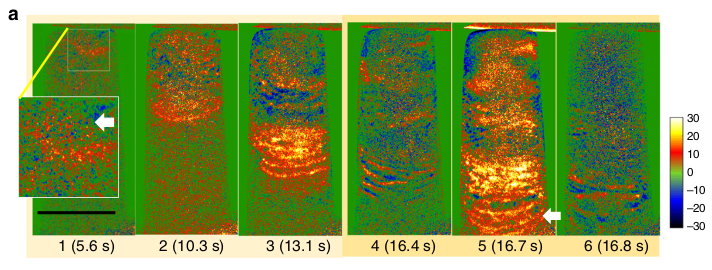
\includegraphics[width=1\textwidth]{./avalanche.png}
  \caption{Dislocation avalanche in a single  $ Al_{0.1}$CoCrFeNi crystal  (Source:Dislocation avalanche mechanism in slowly compressed high entropy alloy nanopillars (Yang Hu et al))}
\end{figure}
\subsubsection{Characteristics of dislocation avalanche in single crystal}
The dislocation avalanches in a single crystal can be characterised by the following properties. The dislocation avalanche in a single crystal is scale invariant,intermittent and the avalanche size distribution follows a power law. The general form of the avalanche strain distribution in a single crystal is given by $ P(s) = Cs^{-\tau} exp[-(\frac{s}{s_0})^2] $ where C is the normalisation constant and $S_0$ is the characteristic strain of the largest avalanches. The avalanche size distribution is unaffected by internal variables like the material and crystal structure and also by the applied stress. During the plastic deformation through bursts the instantaeous strain rate may exceed the average strain rate by several orders of magnitude.
\subsubsection{Dislocation avalanche mechanism in sub-micron plasticity of single crystals}
\indent\indent  For studying the mechanism of dislocation avalanches in sub-micron plasticity nickel nano pillar is considered for the observation. The nanopillar is studied using 3-D discrete dislocation dynamics(DDD) under loading. Since there is not much slip planes and dislocations in sub-micron level the hardening depends on the size of the specimen chosen. When observed using DDD the nano pillar showed the creation and destruction of dipolar loops. A jogged dislocation can turn into a full dipolar-loop following the classical Johnston-Gilman mechanism. When the stress reaches a value that is large enough to bow-out the dislocation segment with the most favourable shear stress dipolar loops starts to grow. When the stress reaches the first yield point different dislocation segments interact with each other and the boundary leaving behind trail of debris. As a result, the nanopillar is in nearly starved condition. The applied stress increases in order to keep up with the strain rate. When the stress reaches a critical value, the debris become the source of new dislocation loops. The fresh dislocation segments continue to expand at fast rate as result of this the stress value drops and the process happens in cyclic manner. Since dipolar loops are continually formed and destroyed it results in the formation of strain avalanches with different amplitudes and distributions. The figure(2) shows the rise and drop of the stress with increasing strain. It is also found that the strain avalanches are found to be dependant on dislocation density. Figure(2) shows the increase in strain oscillations with decrease in dislocation density. But this above phenomenon tends to have no effect on the universal size distribution of avalanches.
\begin{figure}[htbp]
  \centering
  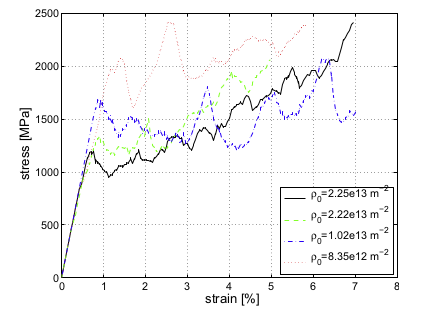
\includegraphics[width=1\textwidth]{./2.png}
  \caption{Stress-strain curve of sub-micron plasticity in FCC-metals (Source:The origin of strain avalanches in sub micron plasticity of FCC metals (Tamer Crosby et al))}
\end{figure} 
\subsubsection{Effect of temperature on dislocation avalanches in single crystal}
\indent\indent In order to find the effect of temperature on dislocation avalanches uniaxial compression tests are carried out on ice crystal from -20 to $ -3^0 $C. An increase of temperature favours the diffusion of vacancies within the crystal and consequently dislocation climb. Also the lattice friction decreases with increase in temperature. So the velocity of the moving dislocations increases with increase in temperature. As a result of this, the relaxation time of the dislocation avalanches decreases gradually. When the dislocation reches certain velocity drag resistance come into play because of the interaction between moving dislocations and excitations such as phonons. Even though the temperature affects the behaviour of individual dislocations like the velocity and relaxation time, it does not affect the universal size distribution of the avalanches.
\newpage

\end{document}